
\mode<presentation>
{
	\usetheme{Grame}
	\setbeamercovered{transparent}
%   \setbeamertemplate{background}{\includegraphics[width= \paperwidth]{imgs/grame}}
	\setbeamertemplate{footline}{{\centering \includegraphics[height=0.5cm]{imgs/logograme}\\ \vspace{1mm}}} 
	\setbeamertemplate{navigation symbols}{} 
	\setbeamerfont{frametitle}{size=\large,series=\bfseries} 
}

\usepackage[utf8]{inputenc}
\usepackage{times}
\usepackage{hyperref}
\hypersetup{
	colorlinks=true,
	linkcolor=black,
	urlcolor=blue
}

%\includeonlyframes{current}

\newcommand{\breathe}		{\vspace{2mm}}
\newcommand{\emptyseg}	{\ensuremath{\oslash}}
\newcommand{\seg}[1]		{Seg(#1)}

\newcommand{\colornote}	{\color[rgb]{0.4,0.4,0.4}}
\newcommand{\coloremph}	{\color[rgb]{0.765,0.184,0}}
\newcommand{\lcolorb}[1]	{\color<#1>[rgb]{0,0,1}}
\newcommand{\lcolort}[1] {#1} %{\color<#1>[rgb]{0.5,0,0}}
\newcommand{\mapdef}[1] 	{{\color[rgb]{0.5,0,0} \emph{#1}}}
\newcommand{\mapex}		{\footnotesize \color[rgb]{0.5,0.4,0.4}}
\newcommand{\lra}			{$\leftrightarrow$}

\newcommand{\exgraph}[1]		 {
	\frametitle{\exemple s} 
	\begin{center}
	\includegraphics[width = 80mm]{#1}
	\end{center}
}

\newcommand{\exexpr}[1]		 {
	\begin{columns}
		\begin{column}[l]{80mm}
		#1
		\end{column}
	\end{columns}
}

%-----------------------------------------------------------------
\def\viewer{/Applications/Interlude-0.53/InterludeScoreViewer.app}
%-----------------------------------------------------------------

\ifdefined \frenchversion
\newcommand{\french}[1] 	{#1}
\newcommand{\eng}[1] 		{}

\def\version{Avril 2010}
\def\exemple{Exemple}
\def\implementation{Implémentation}
\def\synchronisation{Synchronisation}
\def\saidempty{est dit vide quand}
\def\ou{ou}
\def\where{où}
\def\graphic{graphique}
\def\reltime{temps relatif}
\def\texte{texte}
\def\score{partition}
\def\vectoriel{vectoriel}
\def\demo{Démo}
\def\et{et}
\def\ffond{fréquence fondamentale}
\def\ksigthick{signal d'épaisseur constant}
\def\ksigcolor{signal de couleur constant}
\def\ksigrms{signal RMS}
\newcommand{\rmsval}[1] 	{valeurs RMS de #1}

\else

\newcommand{\french}[1] 	{}
\newcommand{\eng}[1] 		{#1}

\def\version{April 2010}
\def\exemple{Example}
\def\implementation{Implementation}
\def\synchronisation{Synchronization}
\def\saidempty{is said empty when }
\def\ou{or}
\def\where{where}
\def\graphic{graphic}
\def\reltime{relative time}
\def\texte{text}
\def\score{score}
\def\vectoriel{vectorial}
\def\demo{Demo}
\def\et{and}
\def\ffond{fundamental frequency}
\def\ksigcolor{constant color signal}
\def\ksigthick{constant thickness signal}
\def\ksigrms{RMS signal}
\newcommand{\rmsval}[1] 	{#1 RMS values}

\fi


%-----------------------------------------------------------------
\title{{\huge 
\french{Partitions musicales augmentées}
\eng{Augmented Music Scores}
}}

%\subtitle{\tiny ANR-08-CORD-010}
%\author{Grame}
\institute{D. Fober, C. Daudin, Y. Orlarey, S. Letz \\
\vspace{2mm}
Grame\\ 
Centre national de création musicale \\
Lyon - France
}

\date[Février 2010]{{\scriptsize \version}}

% Delete this, if you do not want the table of contents to pop up at
% the beginning of each subsection:
\AtBeginSection[]
{
  \begin{frame}<beamer>{Sommaire}
    \tableofcontents[currentsection]
  \end{frame}
}

%-------------------------------------------------------------------------
\begin{document}

\frame{\titlepage}

%-----------------------------------------------------------------
\section{Interlude}
%-----------------------------------------------------------------
\subsection{
\french{Le projet Interlude}
\eng{The Interlude Project}
}
\begin{frame}
	\frametitle{\french{Le projet Interlude.} \eng{The Interlude Project.}}
\french{Nouveaux paradigmes numériques pour l'exploration et l'interaction gestuelle expressive avec des contenus musicaux.}
\eng{New digital paradigms for the expressive gestural exploration and interaction with music contents.}
 \\
	\vspace{3mm}
	\onslide<2->
	\begin{block}{\french{Domaines d'applications :}\eng{Application domains:} }<+->
	\begin{itemize}
\french{
	\item professionnel {\mapex(pédagogie, pièces interactives...)}
	\item grand public {\mapex (jeux musicaux...)}
}
\eng{
	\item professional {\mapex(pedagogy, interactive music...)}
	\item general public {\mapex (musical games...)}
}
	\end{itemize}
	\end{block}	

	\onslide<3>
	\vspace{3mm}
	\french{Partenaires :} \eng{Partners:}
	\begin{itemize}
	\item	Ircam, Grame
	\item	 VoxLer, Dafact
	\item	NoDesign, Atelier les Feuillantines
	\end{itemize}
\end{frame}

\begin{frame}
	\frametitle{\french{Interaction avec des contenus symboliques.}
					\eng{Interaction with symbolic content.}}
	
	\begin{block}{\french{Partition musicale augmentée.}\eng{Augmented Music Score}}<+->
	\begin{itemize}
\french{
	\item<+-> {\small Une \emph{partition musicale augmentée} est une partition mettant en relation 
	un objet musical symbolique avec différentes représentations de son interprétation.}	
	\item<+-> {\small La partition musicale est à considérer au sens large, 
	comme un objet graphique permettant de représenter un objet temporel. }
	\item<+-> {\small 	L'interprétation représente une instance 
	sonore ou gestuelle particulière de la partition. }
}
\eng{
	\item<+-> {\small An \emph{augmented music score} is a score that connects a symbolic music object
	to different representations of its performance.}	
	\item<+-> {\small The music score is to be taken in a broad sense, 
	as a graphic object representing a temporal object.}
	\item<+-> {\small The performance corresponds to a specific sound or gesture instance of the score. }
}
	\end{itemize}
	\end{block}
\end{frame}

\begin{frame}
	\frametitle{\french{Problématiques} \eng{Problematics}}	
	\begin{block}{\french{Au coeur de la partition augmentée}
					\eng{The core of the augmented music score}}<+->
	\begin{itemize}
	\breathe
	\french{	\item	extension de la partition à des objets musicaux arbitraires}
	\eng{		\item	score extension to arbitrary music objects}
	\breathe
	\french{	\item 	expression de relations entre espaces graphiques et temporels}
	\eng{		\item 	expression of relations between graphic and time spaces}
	\breathe
	\french{	\item	représentation de l'interprétation (gestuelle, sonore)}
	\eng{		\item	performance representation (gestural, sound)}
	\end{itemize}
	\vspace{5mm}
	\end{block}
\end{frame}


%-----------------------------------------------------------------
\section{\french{Partition augmentée.}\eng{Augmented Music Score}}
%-----------------------------------------------------------------
\subsection{\french{Composants}\eng{Components}}
\begin{frame}
	\frametitle{\french{Objets musicaux de première classe}
				 \eng{First class music objects}}
	\begin{block}{\french{Tous les composants de la partition :}
					\eng{All the score components:} }<+->
	\begin{itemize}
\french{
	\item ont une dimension graphique,
	\item ont une dimension temporelle,
	\item sont adressables aussi bien dans l'espace graphique que temporel,
	\item gèrent les relations entre espace temporel et graphique,
	\item sont synchronisables dans l'espace graphique et temporel.
}
\eng{
	\item have a graphic dimension,
	\item have a time dimension,
	\item can be addressed both in the graphic and time domains,
	\item maintain relations between time and graphic space,
	\item can be synchronized in the time and graphic space.
}
	\end{itemize}
	\end{block}	
\end{frame}

%-------------------------------------------------
\begin{frame}
	\frametitle{\french{Composants}\eng{Components}}
	
	\begin{block}{\french{Typologie des ressources graphiques.}
				   \eng{Graphic resources typology.} }<+->
	\begin{itemize}
\french{
	\item Partitions musicales \\ format GMN (Guido Music Notation format) ou MusicXML
	\item Eléments textuels
	\item Graphiques bitmaps (jpg, gif, tiff, png, ...)
	\item Graphiques vectoriels (rectangles, ellipses, ...)
	\item Représentations graphiques du son et du geste
}
\eng{
	\item Music scores \\ GMN (Guido Music Notation format) or MusicXML format
	\item Textual elements
	\item Graphic bitmaps (jpg, gif, tiff, png, ...)
	\item Vectorial graphic (rectangles, ellipses, ...)
	\item Sound and gesture graphic representations
}
	\end{itemize}
	\end{block}
	
\end{frame}

%-------------------------------------------------
\begin{frame}
	\frametitle{\french{Paramètres de contrôle.}\eng{Available parameters}}
	
	\begin{block}{\french{Paramètres de contrôle communs.}\eng{Common parameters} }<+->
	\begin{itemize}
		\item position (x, y, z)
		\item \french{échelle}\eng{scale}
		\item rotation
		\item \french{couleur}\eng{color}
		\item date
		\item \french{durée}\eng{duration}
		\item \french{visibilité}\eng{visibility}
	\end{itemize}
	\end{block}
\end{frame}

\begin{frame}
	\frametitle{\exemple}
	\vspace{-4mm}
	\begin{center}
	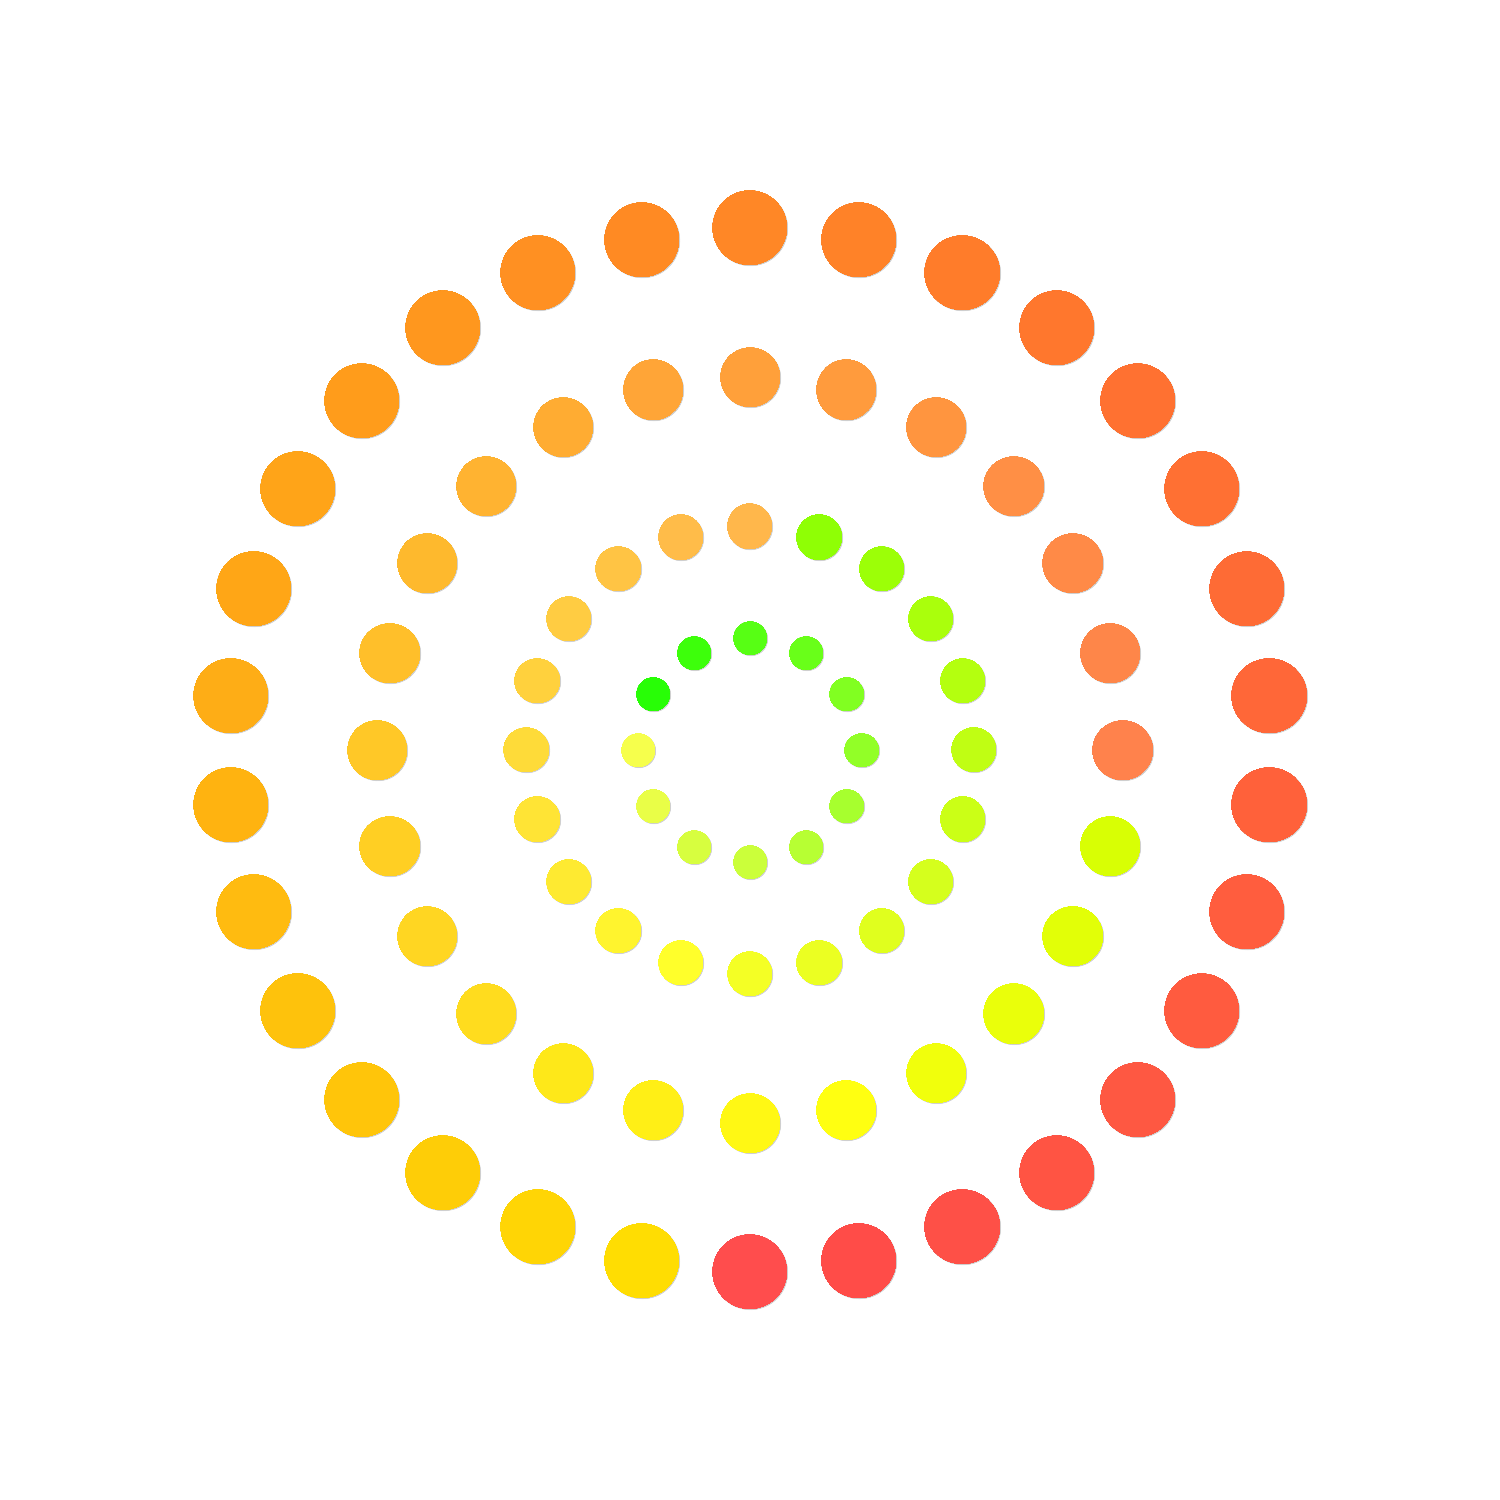
\includegraphics[height = 75mm]{imgs/scene}	
	\end{center}
\end{frame}

%-------------------------------------------------
\subsection{\implementation}
\begin{frame}
	\frametitle{\implementation}
	\begin{itemize}
\french{
	\item sous forme de librairie partagée C++.
	\item sous forme d'application : afficheur de partition augmentée.
	\item multi-platform [MacOS X, Linux, Windows].
	\item basé sur le framework Qt. \includegraphics[height = 5mm]{imgs/Qt}
	\item basé sur le moteur Guido et la librairie libMusicXML.
	\item support du protocole OSC [oscpack].
}
\eng{
	\item as a C++ shared library.
	\item as an application: an augmented score viewer.
	\item multi-platform [MacOS X, Linux, Windows].
	\item based on the Qt framework. \includegraphics[height = 5mm]{imgs/Qt}
	\item based on the Guido engine and the libMusicXML library.
	\item supports the OSC protocol [oscpack].
}
	\end{itemize}
	\begin{center}
	\includegraphics[height = 15mm]{imgs/opensource}
	\end{center}
\end{frame}


%-----------------------------------------------------------------
\section{\synchronisation}
%-----------------------------------------------------------------
\subsection{\french{Segments et segmentations}
			  \eng{Segments and segmentations}}
\begin{frame}
	\frametitle{\french{Segments temporels}\eng{Time segments}}
	\begin{columns}
		\begin{column}[c]{4cm}
		\includegraphics<1->[height = 8mm]{imgs/segment1D} 
		\end{column}
		\begin{column}[c]{4cm}
		\includegraphics<3->[height = 8mm]{imgs/segments1DI}
		\end{column}
	\end{columns}

%	\begin{center} \includegraphics[height = 8mm]{imgs/segment1D} \end{center}
%	\vspace{4mm}
	\begin{itemize}
	\item<1-> 	\french{Un \emph{segment temporel} est défini comme un intervalle}
		\eng{A \emph{time segment} is defined as an interval}
 		$i=[t_{0},t_{1}[$ \french{tel que}\eng{such as} $t_{0} \leqslant t_{1}$.

	\item<2-> $i=[t_{0},t_{1}[$ \saidempty $t_{0} = t_{1}$.\\ 
		\french{Il sera noté \emptyseg.} \eng{We will use \emptyseg\ to denote empty intervals.}

	\item<3-> 
		\french{L'intersection de 2 segments temporels est le plus grand intervalle tel que :}
		\eng{Time  segments intersection is the largest interval such as:}
\[ \forall i_{m},\ \forall  i_{n}, 
\ i_{m} \cap i_{n}  := \{ j \ |\ j \in i_m \ \land\ j \in i_n \}
\]
	\end{itemize}
\end{frame}

\begin{frame}
	\frametitle{\french{Segments graphiques}\eng{Graphic segments}}	
	\begin{columns}
		\begin{column}[c]{4cm}
		\includegraphics<1->[height = 24mm]{imgs/segment2D} 
		\end{column}
		\begin{column}[c]{4cm}
		\includegraphics<3->[height = 24mm]{imgs/segments2DI}
		\end{column}
	\end{columns}
		
	\begin{itemize}
	\item<1-> 	
	\french{Un \emph{segment graphique} $g$ est défini comme un rectangle donné par deux intervalles $g=(x,y)$ où $x$ est un intervalle sur l'axe des abscisses et $y$, sur l'axe des ordonnées.}
	\eng{A \emph{graphic segment} $g$ is defined as a rectangle given by two intervals $g=(x,y)$ where $x$ is an interval on the x-axis and $y$, on the y-axis.}

	\item<2-> $g=\{x,y\}$ \saidempty $x = \emptyseg $ \ou\ $y = \emptyseg $

	\item<3-> Intersection $\cap$ \french{entre segments graphiques :}\eng{between graphic segments:}
\[ \forall g_{m}=\{x_{m},y_{m}\},\ \forall  g_{n}=\{x_{n},y_{n}\},\ 
g_{m} \cap g_{n} = \{x_{m} \cap x_{n}, y_{m} \cap y_{n}\}
\]
	\end{itemize}
\end{frame}

\begin{frame}
	\frametitle{\french{Généralisation de la notion de segment}
				  \eng{Segment generalization}}
	\begin{itemize}
\french{
	\item<+-> 	Un segment de dimension $n$, noté $s^n$, est défini comme une liste de $n$ intervalles $s^n=(i_1,...,i_n)$ où $i_j$ est un intervalle sur la dimension $j$.
	\item<+-> 	Un segment $s^n$ de dimension $n$ est dit vide quand\ $\exists i \in s^n\ |\ i = \emptyseg $.
	\item<+-> 	L'intersection de segments de dimension $n$ est définie comme la liste des intersections de leurs intervalles :
}
\eng{
	\item<+-> 	A $n$-dimensional segment is defined as a set of $n$ intervals $s^n=\{i_1,...,i_n\}$ where $i_j$ is an interval on the dimension $j$.
	\item<+-> 	A segment $s^n$ is said empty when $\exists i \in s^n\ |\ i = \emptyseg $
	\item<+-> Intersection between segments is defined as the set of their intervals intersection:
}
\[ s_1^n \cap s_2^n = (i_1 \cap j_1, ... , i_n \cap j_n)
\]
\where\ $s_1^n = (i_1, ... , i_n)$ et  $s_2^n = (j_1, ... , j_n)$
	\end{itemize}
\end{frame}

%-----------------------------------------------------------------
\begin{frame}
	\frametitle{Segmentations}	
	\begin{itemize}
\french{
	\item<+-> Une ressource $R$ de dimension $n$ est dite \emph{segmentable} quand elle peut être vue comme un segment $S^n$ de dimension $n$.
	\item<+-> La segmentation d'une ressource $R$ est l'ensemble des segments $\seg{R}=\{ s_1^n, ... s_i^n\}$ tels que :
}
\eng{
	\item<+-> A $n$ dimensions resource $R$ is \emph{segment-able} when it can be defined by a segment $S^n$ of dimension $n$.
	\item<+-> The segmentation of a resource $R$ is the set of segments $\seg{R}=\{ s_1^n, ... s_i^n\}$ such as:
}
\[
\begin{array}{rll}
\forall i, j \in \seg{R} & i \cap j =  \emptyseg  & ${\footnotesize \french{les segments sont disjoints}\eng{segments are disjoints}}$ \\
\forall i \in \seg{R} & i \cap S^n = i & ${\footnotesize \french{tous les segments sont inclus dans}\eng{all segments are included in} R}$ \\
\end{array}
\]
	\end{itemize}
\end{frame}

%-----------------------------------------------------------------
\subsection{Mappings}
\begin{frame}
	\frametitle{Mapping (1)}		
	\begin{center}
	\french{Un \mapdef{mapping} est une relation entre 2 segmentations.}
	\eng{A \mapdef{mapping} is a relation between 2 segmentations.}
	\includegraphics[width = 70mm]{imgs/patates}	
	\end{center}
	
\end{frame}

\begin{frame}
	\frametitle{Mapping (2)}		
	\begin{columns}
		\begin{column}[l]{75mm}
			\begin{itemize}
			\item<1-> {\small \french{Pour un}\eng{For a} mapping $M\subseteq \seg{R_{1}}\times \seg{R_{2}}$ 
				\french{la fonction }\eng{the function}:
			\[ M^{+}(i)=\{ i'\in \seg{R_{2}}\ |\ (i,i')\in M\}\]
			\french{donne l'ensemble des segments de $R_{2}$ associés au segment $i$ de $R_{1}$}
			\eng{gives the set of segments from $R_{2}$ associated to the segment $i$ from $R_{1}$.}
			}
			\item<2-> {\small \french{et la fonction inverse }\eng{and the reverse function}: 
			\[ M^{-}(i')=\{ i \in \seg{R_{1}}\ |\ (i,i') \in M\}\]
			\french{donne l'ensemble des segments de $R_{1}$ associés au segment $i'$ de $R_{2}$.}
			\eng{gives the set of segments from $R_{1}$ associated to the segment $i'$ from $R_{2}$.}
			}
			\end{itemize}
		\end{column}
		\begin{column}[l]{40mm}
			\includegraphics<1>[width=40mm]{imgs/patates-dr}		
			\includegraphics<2>[width=40mm]{imgs/patates-rr}		
		\end{column}
	\end{columns}
\end{frame}

%-----------------------------------------------------------------
\begin{frame}
	\frametitle{Mapping (3)}		
	\begin{columns}
		\begin{column}[l]{75mm}
		\begin{itemize}
		\item<1-> {\small 
		\french{Ces fonctions sont définies sur un ensemble de segments comme l'union des mappings de chaque segment :}
		\eng{These functions are defined for a set of segments as the union of each segment mapping:}
		\[ M^{+}(\{i_1, ...i_n\})= M^{+}(i_1) \cup M^{+}(i_2) ...  \cup M^{+}(i_n)\]}
	%et
	%	\[ M^{-}\{i_1, ...i_n\}=\{ M^{-}(i_1), ..., M^{-}(i_n) \}\]

		\item<2->{\small \french{Composition de mappings :}\eng{Mappings composition:}\\
		\french{soit}\eng{let} $M_{1}\subseteq \seg{R_{1}}\times \seg{R_{2}}$ \\
		\et\ $M_{2}\subseteq \seg{R_{2}}\times \seg{R_{3}}$
		\[ (M_{1} \circ M_{2})^{+}(i) = M_2^{+}(M_1^{+}(i))\]}
		\item<3->{\small \french{soit la relation }\eng{i.e. the relation}:
		\[ M_{1} \circ M_{2} \subseteq \seg{R_{1}}\times \seg{R_{3}} \]}
		\end{itemize}
		\end{column}
		\begin{column}[l]{40mm}
			\includegraphics<1>[width=40mm]{imgs/patates-vr}		
			\includegraphics<2>[width=30mm]{imgs/patates-cr}		
			\includegraphics<3>[width=31mm]{imgs/patates-crd}		
		\end{column}
	\end{columns}
\end{frame}

\begin{frame}
	\frametitle{\french{Relations entre espaces graphiques et temporels}	
				  \eng{Relations between graphic and time spaces.}}

\french{Segmentations et mappings pour chaque type de composant.}
\eng{Segmentations and mappings for each component type.}
\\
\vspace{5mm}
\begin{tabular}{|r|l|}
\hline
type & \french{segmentations et mappings requis} \eng{segmentations and mappings required} \\
\hline
{\small \texte}		& {\small \textit{\graphic} \lra\ \textbf{text  \lra\ \reltime}} \\
{\small \score}	& {\small \textit{\graphic \lra\ \french{\reltime enroulé}\eng{wrapped \reltime}} \lra\ \textit{\reltime}} \\
{\small image	}	& {\small \textit{\graphic} \lra\ \textbf{pixel \lra\ \reltime}} \\
{\small gr. \vectoriel}	&  {\small \textbf{\vectoriel \lra\ \reltime}} \\
{\small signal}	&  {\small \textit{\graphic} \lra\ \textbf{frame \lra\ \reltime}} \\
\hline
\end{tabular}
\end{frame}


\begin{frame}
	\vspace{10mm}
	\begin{center}
	{\color[rgb]{0.5,0,0}{\Huge \demo}}
	\end{center}

	\french{Voir }\eng{See}: \\
	\begin{itemize}
	\item \href{/Applications/Interlude-0.53/Max/sync/sync.maxpat}{Max/sync/sync.maxpat}
	\item \href{/Applications/Interlude-0.53/PureData/sync/sync.pd}{PureData/sync/sync.pd}
	\item \href{/Applications/Interlude-0.53/python/example.py}{python/example.py}
	\item \href{/Applications/Interlude-0.53/lisp/example.lisp}{lisp/example.lisp}
	\end{itemize}
	\href{\viewer}{InterludeScoreViewer} 
	\french{doit être actif}\eng{must be running}.
\end{frame}

%-----------------------------------------------------------------
\section{\french{Signaux graphiques}\eng{Graphic signals}}
%-----------------------------------------------------------------
\subsection{\french{Signaux graphiques}\eng{Graphic signals}}
\begin{frame}
	\frametitle{\french{Le problème...}\eng{The problem...}}	
	\french{Approche précédente :}\eng{Previous approach:}
	\includegraphics<1->[width=110mm]{\french{imgs/signalv1}\eng{imgs/signalv1en}}
	\begin{itemize}
	\item<2-> \french{représentations statiques du signal}\eng{static signal representation}
	\item<2-> \french{non extensible dynamiquement}		\eng{non-extensible dynamically}
	\end{itemize}
	
	\vspace{4mm}
	\onslide<3->
	\french{Et maintenant ?}\eng{Currently...}
	\begin{itemize}
	\item \french{système plus général i.e. permettant de couvrir une grande variété de représentations}
			\eng{a more general system, covering a large set of representations}
	\item \french{système extensible dynamiquement}	\eng{dynamically extensible}
	\item \french{et facile à utiliser...}				\eng{and easy to use...}
	\end{itemize}
\end{frame}

\begin{frame}
	\frametitle{\french{Des signaux graphiques...}\eng{Graphic signals}}
	\begin{block}{\french{Le \mapdef{graphique d'un signal} vu comme un \mapdef{signal graphique}:}
					\eng{The \mapdef{graphic of a signal} as a \mapdef{graphic signal}:}}<+->
\french{Un signal composite constitué :}\eng{A composite signal made of:}
	\begin{itemize}
	\item \french{d'un signal d'élévation (les valeurs en y)}	\eng{a $y$ signal}.
	\item \french{d'un signal d'épaisseur}						\eng{a thickness signal}.
	\item \french{d'un signal de couleur}						\eng{a color signal}.
	\end{itemize}
	\begin{center}
	\includegraphics[width = 60mm]{imgs/graph}	
	\end{center}
	\end{block}
\end{frame}

\begin{frame}
	\frametitle{\french{Des signaux graphiques...}\eng{Graphic signals}}
	\begin{columns}
		\begin{column}[l]{75mm}
		\french{Considérons maintenant que nous disposons d'un signal $S$  défini comme une fonction du temps :}
		\eng{Consider a signal $S$  defined as a time function:}
		\[f(t)  : \mathbb{R} \rightarrow \mathbb{R}^3 =  (y, h, c)\ |\ y, h, c \in \mathbb{R} \]
		\french{alors ce signal pourrait être dessiné directement. \\
		{\small (i.e. sans calcul supplémentaire)}}
		\eng{this signal could be directly drawn.\\
		{\small (i.e. without additional computation)}}		

		\vspace{5mm}
		{\small \colornote \french{Pour simplifier, on suppose que l'espace de couleurs adressé par $c$ n'a qu'une dimension.}
							 \eng{To make simple, we assume that the color space addressed by $c$ has one dimension.}}
		\end{column}
		\begin{column}[l]{40mm}
			\includegraphics<2>[width=40mm]{imgs/oscilloscope}		
		\end{column}
	\end{columns}
\end{frame}

%-----------------------------------------------------------------
\subsection{\french{Composition de signaux}\eng{Signals composition}}

\begin{frame}
	\frametitle{\french{Types de signaux parallèle}\eng{Parallel signals types}}
	\begin{itemize}
	\item<+-> \french{Type d'un signal de couleur :}	\eng{Color signal type:} \\
	\vspace{-5mm}
	{\scriptsize \colornote (\french{modèle HSBA}\eng{HSBA model} [hue, saturation, brigthness, transparency])}  
		\includegraphics<1->[width=15mm]{imgs/hsb}
		\[c ::= \overrightarrow{(h, s , b, a)} \ |\  h, s , b, a \in \mathbb{R}\] 
	\item<+-> \french{Type d'un signal graphique :}	\eng{Graphic signal type:}
		\[g ::= \overrightarrow{(y, th, h, s , b, a)} \ |\  y, th, h, s , b, a \in \mathbb{R}\]
	\item<+-> \french{Type des signaux graphiques parallèles :} \eng{Parallel graphic signals type}
		\[g^n ::= \overrightarrow{g} \ |\  g \in \mathbb{R}^6\]
	\end{itemize}

\end{frame}


\begin{frame}
	\frametitle{\french{Parallélisation de signaux}\eng{Signals parallelization}}

	\onslide<+->
	\french{Soit $\mathbb{S}$, l'ensemble des signaux $s : \mathbb{N} \rightarrow \mathbb{R}$.}
	\eng{Let $\mathbb{S}$, the set of signals $s : \mathbb{N} \rightarrow \mathbb{R}$.}
	 \\
	\french{Nous définissons une opération \emph{parallèle} '$/$' comme :}
	\eng{We define a \emph{parallel} operation '$/$' as:}
	\[s_{1} / s_{2} / ... / s_{n} : \mathbb{S} \rightarrow \mathbb{S}^n\ |\ s_i \in \mathbb{S} \]

	\onslide<+->
	\bigskip
	\french{Fonction du temps d'un signal parallèle} \eng{Time function of a parallel signal}
	$s^n \in \mathbb{S}^n$ : $\mathbb{N} \rightarrow \mathbb{R}^n$
\[ f(t) = (f_0(t), f_1(t), ... f_n(t))\ |\ f_i(t) :  \mathbb{N} \rightarrow \mathbb{R} \]
\end{frame}


%-----------------------------------------------------------------
\subsection{\exemple s}
\begin{frame}
	\exgraph{imgs/curves/pitch} 
	\exexpr{
		$g = S_{f0}\ /\ k_t\ /\ k_c$ 
		\\ {\mapex $S_{f0}$ : \ffond}
		\\ {\mapex $k_t$ : \ksigthick}
		\\ {\mapex $k_c$ : \ksigcolor}
	}
\end{frame}

\begin{frame}
	\exgraph{imgs/curves/finepitch} 
	\exexpr{
		$g = S_{f0}-S_{fr}\ /\ k_t\ /\ k_c$
		\\ {\mapex $S_{f0}$ : \ffond}
		\\ {\mapex $S_{fr}$ : \french{fréquence de référence}\eng{reference frequency}}
		\\ {\mapex $k_t$ : \ksigthick}
		\\ {\mapex $k_c$ : \ksigcolor}
	}
\end{frame}

\begin{frame}
	\exgraph{imgs/curves/articulation} 
	\exexpr{
		$g = k_y\ /\ S_{rms}\ /\ k_c$ 
	\\ {\mapex $S_{rms}$ : \ksigrms}
	\\ {\mapex $k_y$ : \french{signal $y$ constant}\eng{constant $y$ signal}}
	\\ {\mapex $k_c$ : \ksigcolor}
	}
\end{frame}

\begin{frame}
	\exgraph{imgs/curves/pitchedarticulation} 
	\exexpr{
		$g = S_{f0}\ /\ S_{rms}\ /\ k_c$ 
	\\ {\mapex $S_{rms}$ : \ksigrms}
	\\ {\mapex $S_{f0}$ : \ffond}
	\\ {\mapex $k_c$ : \ksigcolor}
	}
\end{frame}

\begin{frame}
	\onslide<+->
	\exgraph{imgs/curves/pitchedstackedharm} 
	\exexpr{
		{\small $g0 = S_{f0}\ /\ S_{rms0}\ /\ k_c0$}
	\\ {\mapex $S_{f0}$ : \ffond}
	\\ {\mapex $S_{rms0}$ : \rmsval{f0}}
	}
	\exexpr{
	\\ {\small $g1 = S_{f0} \ /\ S_{rms1} + S_{rms0}\ /\ k_c1$}
	\\ {\mapex $S_{rms1}$ : \rmsval{f1}}
	}
	\exexpr{
	\\ {\small $g2 = S_{f0} /\ S_{rms2} + S_{rms1}  + S_{rms0} \ /\ k_c2$}
	\\ {\mapex $S_{rms2}$ : \rmsval{f2}}
	\\ ...
	}
	\exexpr{
	\\	$g = g2 \ /\  g1 \ /\ g0$
	}
\end{frame}


%-----------------------------------------------------------------
\begin{frame}
	\vspace{10mm}
	\begin{center}
	{\color[rgb]{0.5,0,0}{\Huge \demo}}
	\end{center}

	\french{Voir }\eng{See}: \\
	\begin{itemize}
	\item \href{/Applications/Interlude-0.53/Max/sinus/sinus.maxpat}{Max/sinus/sinus.maxpat}
	\item \href{/Applications/Interlude-0.53/PureData/sinus/sinus.pd}{PureData/sinus/sinus.pd}
	\item \href{/Applications/Interlude-0.53/Max/siggraph/siggraph.maxpat}{Max/siggraph/siggraph.maxpat}
	\item \href{/Applications/Interlude-0.53/PureData/siggraph/siggraph.pd}{PureData/siggraph/siggraph.pd}
	\end{itemize}
	\href{\viewer}{InterludeScoreViewer} 
	\french{doit être actif}\eng{must be running}.
\end{frame}



\begin{frame}
	\frametitle{}	
	\begin{center}
	
	\bigskip
	{\color[rgb]{0.5,0,0}{\Huge INScore} \\ 
	\vspace{5mm}
	{\LARGE\french{Partitions augmentées interactives}\eng{Interactive Augmented Scores}}} \\
	\href{http://interlude.ircam.fr/}{http://interlude.ircam.fr/}
	
	\bigskip
	\bigskip
	\includegraphics[width=15mm]{imgs/opensource} \\
	\end{center}
	
\end{frame}


\end{document}


